\subsubsection{Diagrama del modelo de datos}
La figura \ref{fig:diagrama_modelo_social_final} muestra el diagrama con el diseño final del modelo de datos de la zona social.
\begin{landscape}
	\begin{figure}[h]
		\centering
		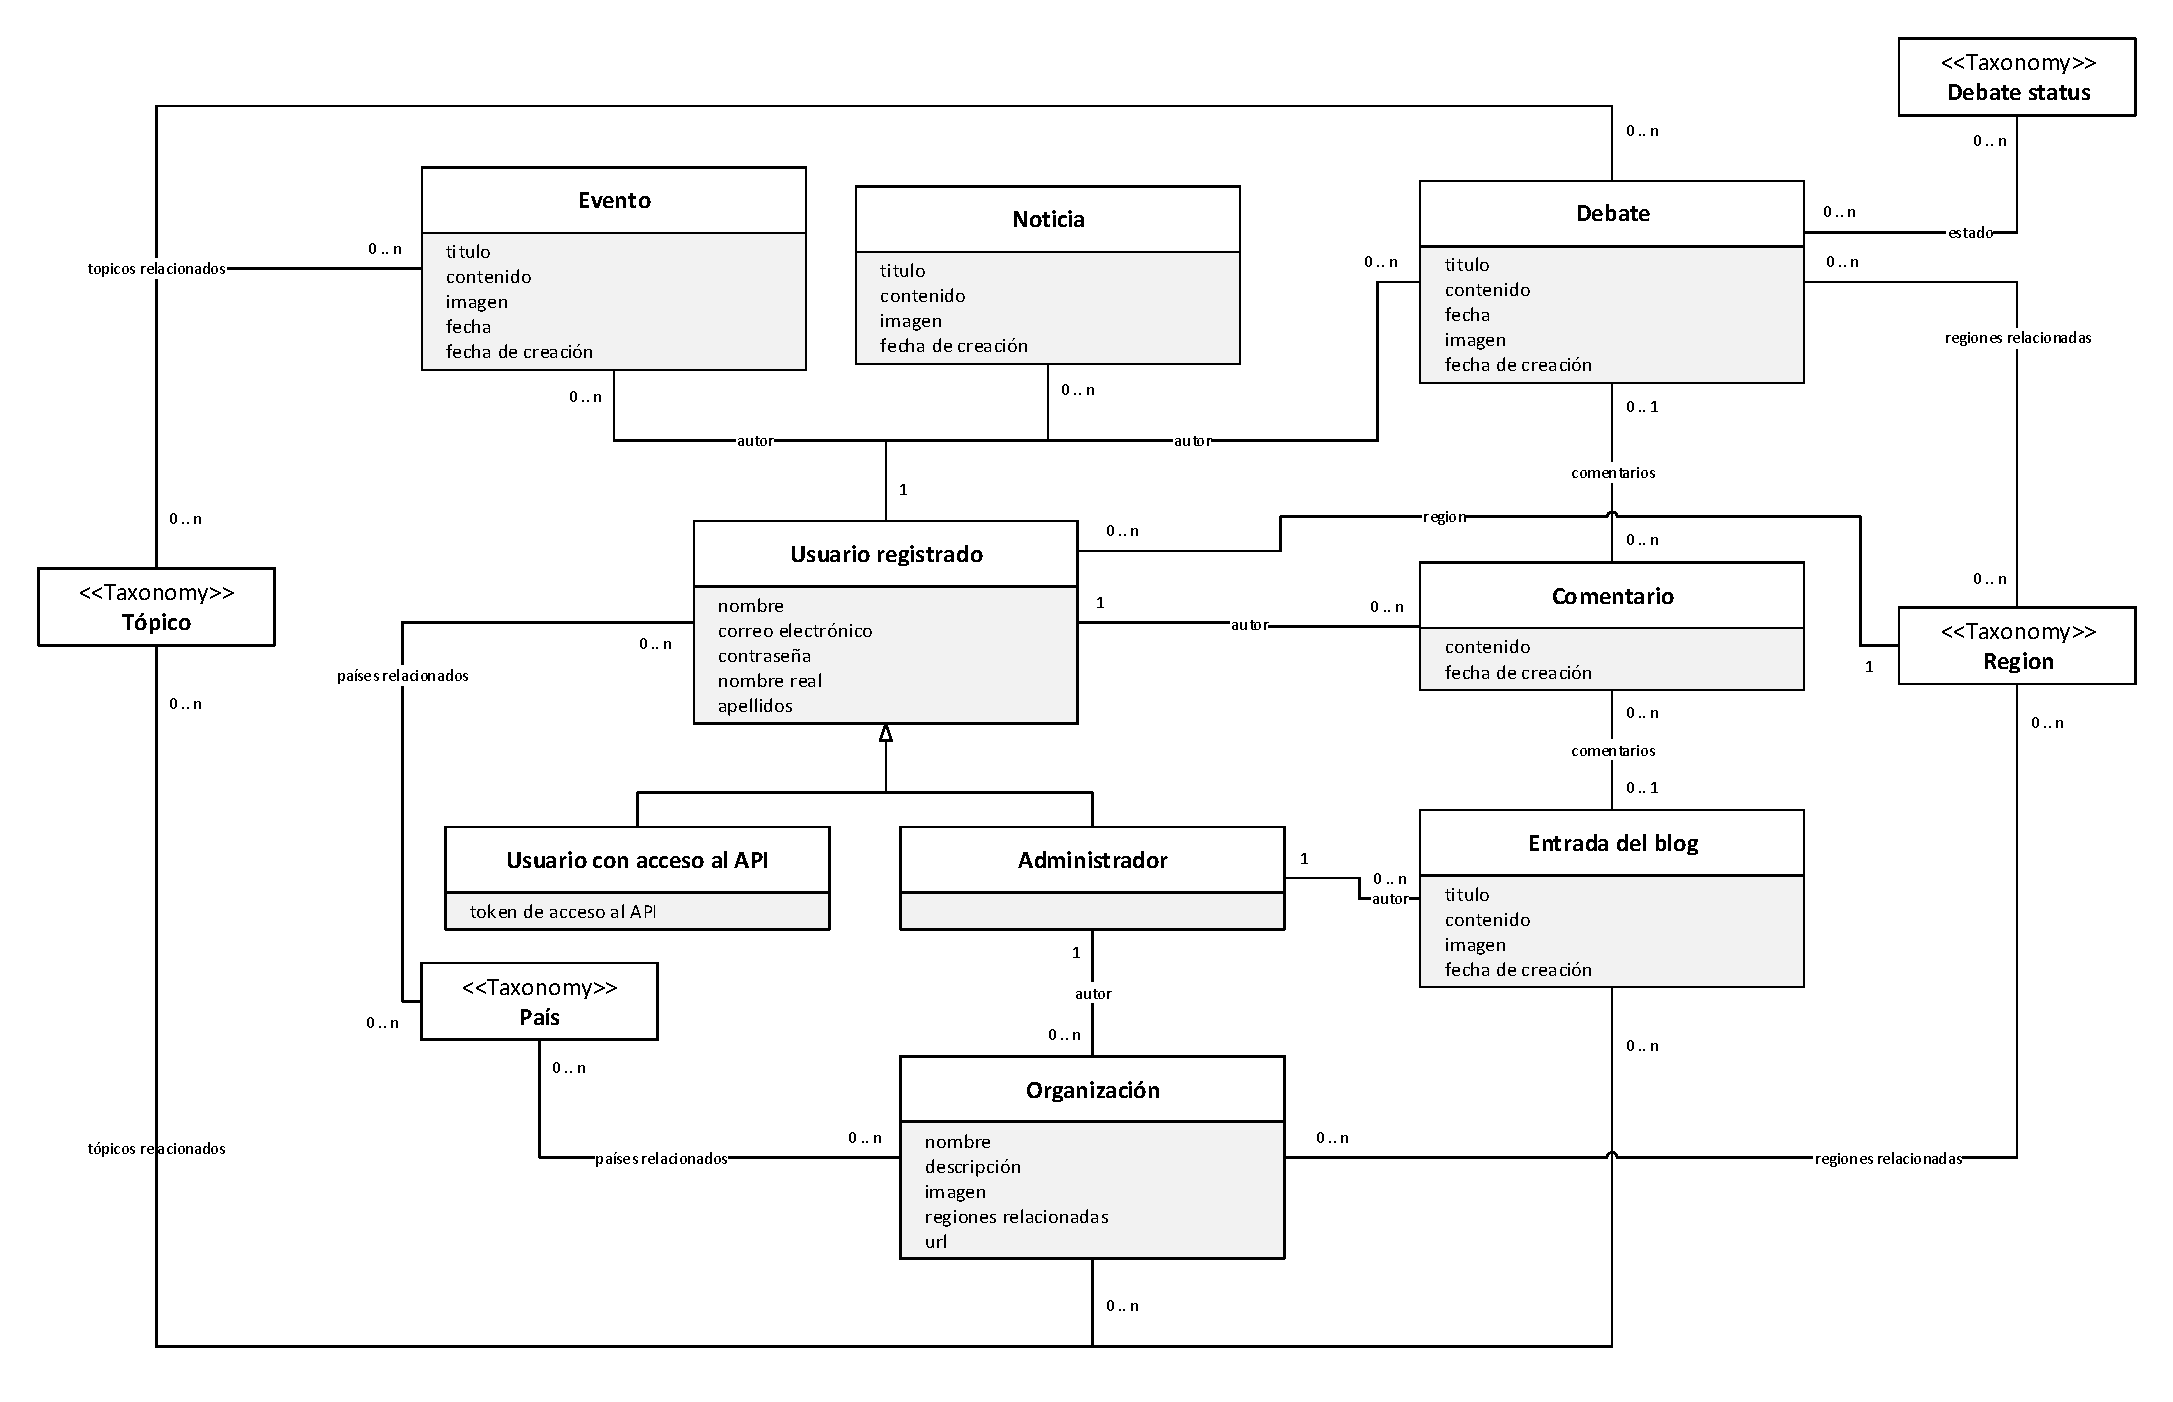
\includegraphics[width=25cm]{clases/clases_debate_final}
		\caption{Diseño final del modelo de datos de la zona social}
		\label{fig:diagrama_modelo_social_final}
	\end{figure}
\end{landscape}

La variación respecto al diseño preliminar de éste modelo que se puede observar en la sección ``\nameref{clases_preliminares_modelo_debate}'' perteneciente al capítulo \ref{chapter04} es mínima y se explicará a continuación:
\begin{itemize}
	\item Los \textbf{tópicos relacionados} de los eventos, debates, organizaciones y entradas del blog han sido extraídos a una taxonomía externa.
	\item Los \textbf{países relacionados} de las organizaciones y usuarios también han sido extraídos a una taxonomía externa.
	\item Al igual que los anteriores, las \textbf{regiones relacionadas} de las organizaciones y los debates también han sido extraídos a una taxonomía externa.
	\item El \textbf{estado} de los debates también pertenece a una taxonomía externa.
\end{itemize}

La razón principal de éstas taxonomías es la capacidad de \textit{enlazar} los diferentes contenidos del portal.  Por ejemplo, ver un elemento de la taxonomía \textit{Tópico} permitirá acceder a todos los eventos, debates, organizaciones y entradas del blog relacionados con dicho término.\\
En cuanto a los debates, la existencia de una taxonomía que represente su estado permite añadir o eliminar nuevos estados de forma sencilla y sin tener que realizar ninguna modificación en los componentes del modelo.

\subsubsection{Elementos del modelo de datos}
A pesar de la inclusión de taxonomías para representar algunos elementos del modelo de datos de la zona social, éste no ha sufrido ninguna variación respecto a lo ya expuesto en la fase de análisis del sistema. Todas las descripciones de campos y elementos realizadas en la sección ``\nameref{clases_preliminares_modelo_debate}'' del capítulo \ref{chapter04} siguen siendo válidas.